% !TEX root = ../NeuralNetworksFR.tex


%%%%%%%%%%%%%%%%%%%%%%%%%%%%%%%%%%%%%%%%%%%%%%%%%%%%%%%%%%
\section{Réseaux de neurones génératifs}

Au lieu d'utiliser des réseaux de neurones pour analyser des images, des travaux de 2014~\cite{goodfellow2014generative} ont montré qu'on pouvait les utiliser \guill{à l'envers} afin de générer des images.
%
Ces réseaux de neurones génératifs trouvent par exemple des applications pour les effets spéciaux, les jeux vidéo et la création artistique. 
%
On retrouve des questions similaires dans l'apprentissage des voitures autonomes et la résolution de jeux de stratégie.
%
La figure~\ref{fig:generative} montre la structure d'un tel réseau $g_{\mygreen{w}}$, qui dépend de poids $\mygreen{w}$. Les couches jouent en quelque sorte des rôles miroirs par rapport à l'architecture des réseaux de neurones discriminatifs exposés dans l'article précédent.
%
A partir d'une entrée ${\color{red}y}$ composée d'un petit nombre de valeurs, qui sont typiquement tirées aléatoirement, on génère une image ${\color{blue} x} = g_{\mygreen{w}}({\color{red}y})$. 

\begin{figure}\centering
	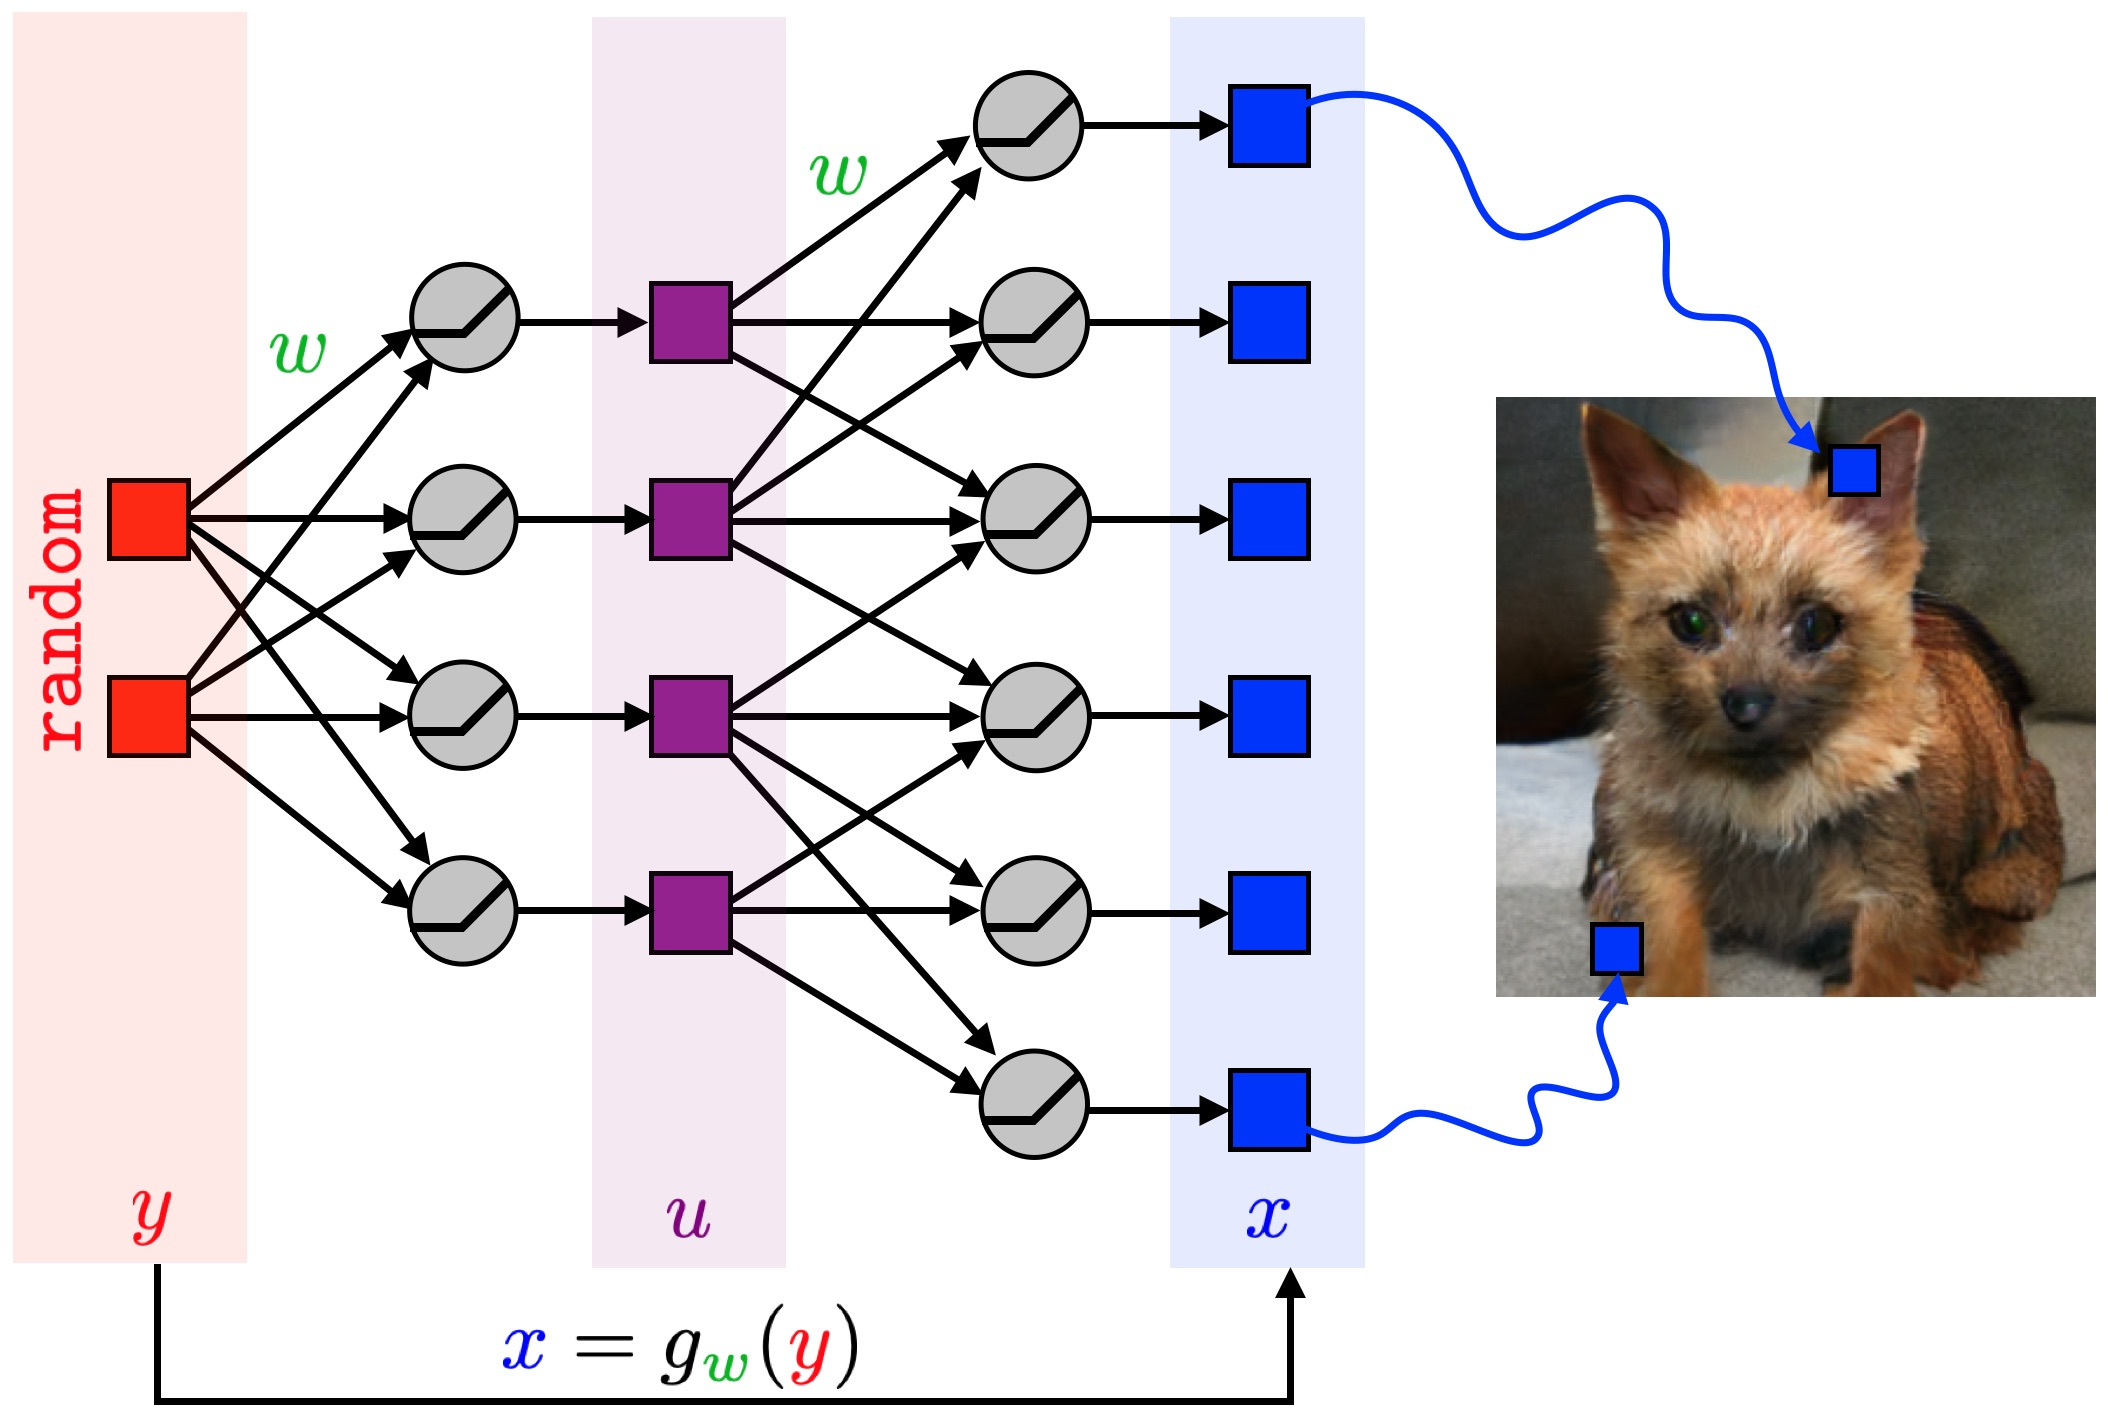
\includegraphics[width=.8\linewidth]{generative}
\caption{\label{fig:generative} Exemple d'un réseau de neurones génératif simplifié (un réseau permettant de générer des images aussi complexes possède plus de couches).  }
\end{figure}

Le problème d'apprentissage de tels réseaux est non-supervisé : on dispose uniquement d'un grand nombre d'images d'apprentissage, sans indication sur ce qu'elles contiennent.
%
Il n'y a plus besoin d'intervention humaine pour indiquer au réseau le contenu des images qu'il doit reconnaitre. 
La collecte de données est ainsi plus simple que pour l'entrainement de réseaux discriminatifs. De plus, ce principe d'apprentissage non supervisé est proche de la façon dont les enfants apprennent, principalement en observant et manipulant le monde qui les entoure.
%
Le but est alors de sélectionner les poids $\mygreen{w}$ des neurones du réseau $g_\mygreen{w}$ de sorte que les images aléatoires générées (les images fausses, \guill{fakes} en anglais) ressemblent le plus possible aux images d'apprentissage. 

%%%%%%%%%%%%%%%%%%%%%%%%%%%%%%%%%%%%%%%%%%%%%%%%%%%%%%%%%%
\section{L'apprentissage non supervisé de réseaux génératifs}
\label{sec-app-gen}

Le but des réseaux de neurones génératifs n'est pas de résoudre une tâche telle que la reconnaissance d'objets dans les images. 
%
Afin d'entrainer les poids $\mygreen{w}$ du réseau, il faut formaliser mathématiquement le problème. Il s'agit de générer un ensemble d'images \guill{virtuelles} (les fausses) qui ressemblent aux images réelles d'une base de données. Il ne s'agit pas simplement qu'une image générée ressemble à une image réelle, il faut mettre en correspondance les deux ensembles d'images. Par exemple, si dans la base de données il y a la moitié d'images de chiens et la moitié d'images de chats, il faut que le réseau génère également pour moitié des chiens et pour moitié des chats. 

On va noter $\{\mylblue{z_1,z_2,\ldots,z_n}\}$ l'ensemble des $n$ images de la base de données. Le nombre $n$ d'images est très grand, de l'ordre de plusieurs milliers ou millions. Etant donné un réseau de neurones génératif $g_{\mygreen{w}}$, qui est paramètré par ses poids $\mygreen{w}$, on note $\{\myblue{x_1,x_2,\ldots,x_n}\}$ un ensemble de $n$ images \guill{fausses} générées aléatoirement par le réseau. Pour générer la première image fausse $\mylblue{x_1}$, ceci signifie que l'on tire aléatoirement les valeurs d'entrée ${\color{red}y_1}$ et qu'on applique le réseau à ces entrées, pour obtenir l'image virtuelle $\mylblue{x_1} = g_{\mygreen{w}}({\color{red}y_1})$. On a ensuite fait la même chose avec $\mylblue{x_2} = g_{\mygreen{w}}({\color{red}y_2})$ et ainsi de suite. 

Le but de l'apprentissage non supervisé est donc de trouver des poids $\mygreen{w}$ de sorte que l'ensemble des fausses images $\{\myblue{x_1,\ldots,x_n}\}$ soit le plus proche de l'ensemble des images $\{\mylblue{z_1,\ldots,z_n}\}$  de la base de données. Le problème d'optimisation s'écrit ainsi 
\eq{
	\umin{\mygreen{w}} \text{Distance}( 
		\{\myblue{x_1,\ldots,x_n} \}, 
		\{\mylblue{z_1,\ldots,z_n}\}  ).
}
Il faut ici se rappeler que les images générées $\{\myblue{x_1, \ldots, x_n} \}$ dépendent du réseau $g_{\mygreen{w}}$ et donc des poids $\mygreen{w}$. On peut reformuler le problème précédent comme
\eq{
	\umin{\mygreen{w}} \text{Distance}( 
		\{g_{\mygreen{w}}({\color{red}y_1}),\ldots, g_{\mygreen{w}}({\color{red}y_n})\}, 
		\{\mylblue{z_1,\ldots,z_n}\}  ).
}
%
La question mathématique qui se pose est donc de définir une notion de distance entre deux ensembles de points. Il existe de nombreuses façons de le faire, et nous allons en expliquer une qui est bien adaptée à ce problème d'apprentissage. 
%
Elle exploite la théorie du transport optimal.


%%%%%%%%%%%%%%%%%%%%%%%%%%%%%%%%%%%%%%%%%%%%%%%%%%%%%%%%%%
\section{Le transport optimal de Monge}
\label{sec-ot}

Le problème de transport optimal est formulé par Gaspard Monge~\cite{Monge1781} en 1781, pour des applications militaires. 
%
La question posée est de déterminer la façon la plus économe de transférer des objets  depuis un ensemble de sources  $\{\myblue{x_1,\ldots,x_n}\}$ vers un ensemble de destinations $\{\mylblue{z_1,\ldots,z_n}\}$. Pour Monge, il s'agit de transférer de la terre depuis des déblais pour créer des remblais. Mais cette question trouve une multitude d'applications. 
%
Pour le problème d'entrainement de réseaux génératifs, les sources sont les images fausses générées par le réseau et les destinations sont les images de la base de données.

\newcommand{\perm}[1]{s_{#1}}


Il faut ainsi relier chaque source, par exemple $\myblue{x_1}$ vers un unique point de destination, que l'on va noter $\mylblue{z_{\perm{1}}}$, où $\perm{1}$ est un entier entre $1$ et $n$. De manière similaire, ${\color{blue}x_2}$ est relié à $\mylblue{z_{\perm{2}}}$ et ainsi de suite. Par exemple, à la figure~\ref{fig:otmonge}, on a relié $\myblue{x_2}$ à $\mylblue{z_5}$, ce qui signifie que $\perm{\myblue{2}}=\mylblue{5}$.
%
Il faut également que chacune des $n$ destinations soit approvisionnée par une source. Ceci signifie par exemple que ${\color{blue}x_1}$ et ${\color{blue}x_2}$ ne peuvent pas être reliés à la même destination, il faut relier toutes les sources à des destinations différentes. Ceci signifie que $\{\perm{1},\ldots,\perm{n}\}$ doit être une permutation des $n$ premiers nombres entiers. 
%
Par exemple, sur la figure~\ref{fig:otmonge}, sur un exemple simple avec $n=6$ éléments, on a choisit sur la gauche la permutation 
\eq{
	(\perm{\myblue{1}}=\mylblue{1},
	\perm{\myblue{2}}=\mylblue{5},
	\perm{\myblue{3}}=\mylblue{4},
	\perm{\myblue{4}}=\mylblue{6},
	\perm{\myblue{5}}=\mylblue{3},
	\perm{\myblue{6}}=\mylblue{2}).
}
%
Le problème de Monge consiste alors à trouver la permutation qui minimise la somme des coûts de transport. Monge a décidé que le coût de transport entre une source $\myblue{x}$ et une destination $\mylblue{z}$ est égal à la distance euclidienne $\norm{\myblue{x} - \mylblue{z}}$ entre les deux points, mais on peut choisir un autre coût : par exemple un temps de trajet ou bien le prix nécessaire en essence si on utilise des camions, etc. On doit ainsi résoudre le problème 
\eq{
	\umin{\text{permutation } s} 
		\norm{\myblue{x_1} - \mylblue{z_{\perm{1}}}} + 
		\norm{\myblue{x_2} - \mylblue{z_{\perm{2}}}} + 
		\ldots + 
		\norm{\myblue{x_n} - \mylblue{z_{\perm{n}}}}.
}
Une fois que l'on a calculé une permutation $s^\star=(\perm{1}^\star,\ldots,\perm{n}^\star)$ optimale (c'est-à-dire qui est solution du problème précédent), on définit la distance entre les ensembles de points comme la valeur du cout total de transport
\eq{
	\text{Distance}( 
		\{\myblue{x_1,\ldots,x_n} \}, 
		\{\mylblue{z_1,\ldots,z_n}\}  ) 
	\eqdef 
		\norm{\myblue{x_1} - \mylblue{z_{\perm{1}^\star}}} + 
		\norm{\myblue{x_2} - \mylblue{z_{\perm{2}^\star}}} + 
		\ldots + 
		\norm{\myblue{x_n} - \mylblue{z_{\perm{n}^\star}}}.
}

\begin{figure}\centering
	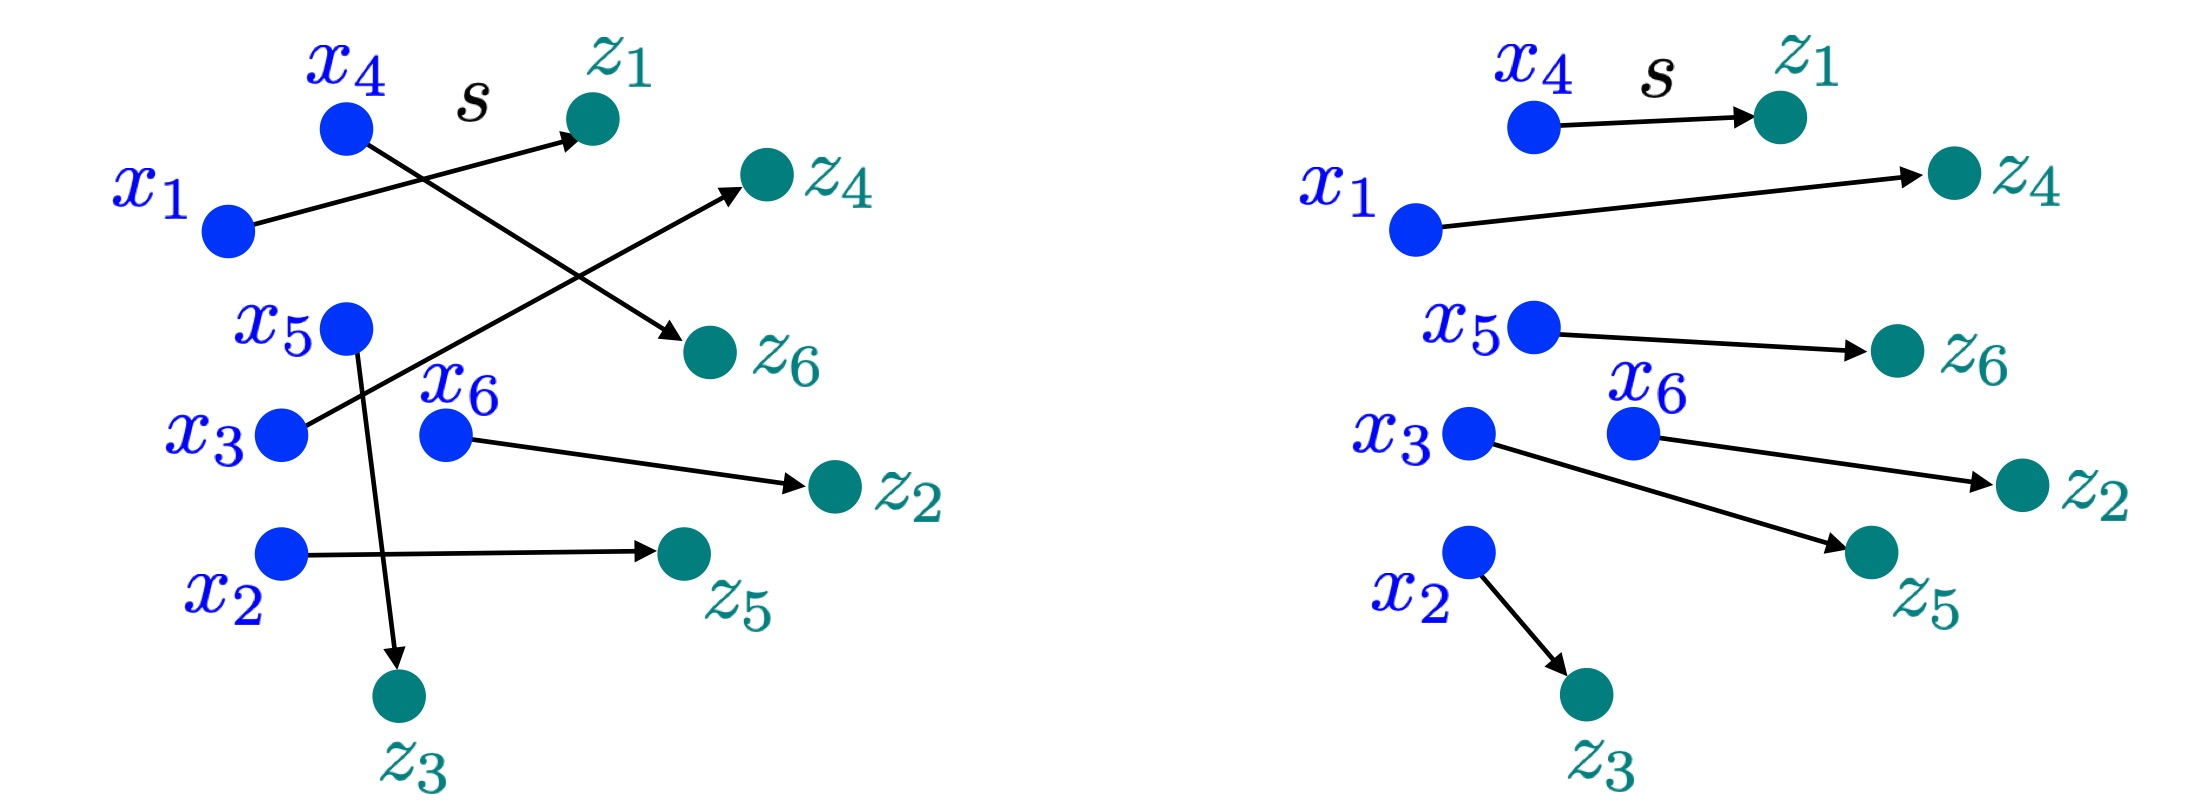
\includegraphics[width=.8\linewidth]{otmonge.jpg}
\caption{\label{fig:otmonge} Exemple à gauche d'une permutation $s$ non-optimale et à droite de la permutation optimale, dans le cas de $6$ points en dimension 2.  }
\end{figure}

La difficulté pour calculer cette distance est que le nombre total de permutations à tester est très grand. En effet, pour le choix de $\perm{1}$ il y a $n$ possibilités, pour celui de $\perm{2}$ il en y a $n-1$ (puisque la valeur de $\perm{1}$ est prise), pour $\perm{2}$ il y en a $n-2$, etc. Donc le nombre total de permutations est égal à $n!$, la factorielle du nombre $n$, qui est définie comme
\eq{
	n! = n \times (n-1) \times (n-2) \times \ldots \times 2 \times 1.
}
Pour $n=6$ comme à la figure~\ref{fig:otmonge}, il y a donc 
\eq{
	6!=6 \times 5 \times 4 \times 3 \times 2 \times 1 = 720 \text{ permutations possibles.}
}
Dans ce cas simple, on peut toutes les tester et choisir la meilleure, qui est, comme montré à la droite de la figure~\ref{fig:otmonge}, 
\eq{
	(\perm{\myblue{1}}=\mylblue{4},
	\perm{\myblue{2}}=\mylblue{3},
	\perm{\myblue{3}}=\mylblue{5},
	\perm{\myblue{4}}=\mylblue{1},
	\perm{\myblue{5}}=\mylblue{6},
	\perm{\myblue{6}}=\mylblue{2}).
}
La difficulté est que pour $n=70$, il y a plus de $10^{100}$ possibilités, ce qui est à comparer aux $10^{79}$ atomes dans l'univers \ldots Et pour entrainer des réseaux de neurones, $n$ est encore beaucoup plus grand ! 
%
Il a donc fallu attendre plusieurs révolutions mathématiques et algorithmiques pour pouvoir obtenir une méthode permettant de résoudre ce problème. 


%%%%%%%%%%%%%%%%%%%%%%%%%%%%%%%%%%%%%%%%%%%%%%%%%%%%%%%%%%
\section{Le transport optimal de Kantorovitch}
\label{sec-kanto}

Monge a remarqué que les solutions de son problème ont des structures très particulières. Par exemple, on peut observer sur la figure~\ref{fig:otmonge}, à droite, que les trajets optimaux ne se croisent pas, et Monge l'avait prouvé dans son article~\cite{Monge1781}. Mais ceci n'est pas suffisant pour résoudre le problème, car il existe encore énormément de trajectoires sans croisement. Il a fallu plus de 200 ans pour comprendre comment obtenir plus d'information sur les solutions afin de les calculer efficacement. 
%
C'est Leonid Kantorovitch qui a trouvé en, 1942~\cite{Kantorovich42}, une nouvelle formulation du problème de transport optimal calculable rapidement. Il a autorisé chaque source à se diviser en plusieurs parties, par exemple deux parties égales avec une pondération de 1/2 chacune. Cette division de la production est intéressante car elle simplifie le problème d'optimisation. Elle est également naturelle pour les préoccupations de Kantorovitch qui était de modéliser et planifier la production en économie. Il a d'ailleurs obtenu le prix Nobel d'économie pour cette idée. 
%
Conjointement à ces travaux pionniers de Kantorovitch, George Dantzig a trouvé en 1947 l'algorithme du simplexe~\cite{dantzig1990origins}, qui permet de résoudre efficacement des problèmes de transport de grande taille. Sa complexité numérique pour résoudre un problème de transport optimal entre $n$ points est de l'ordre de $n^3 = n \times n \times n$, ce qui est beaucoup plus faible que $n!=n \times (n-1) \times \ldots \times 2 \times 1$. Il est au c\oe{}ur d'un très grand nombre de systèmes industriels qui doivent optimiser l'adéquation entre des moyens de production et de consommation. Et on peut du coup également l'utiliser pour entrainer des réseaux de neurones génératifs ! On pourra regarder~\cite{PeyreCuturi} pour plus de détails sur la théorie du transport optimal, les algorithmes efficaces et ses applications à la science des données. 


%%%%%%%%%%%%%%%%%%%%%%%%%%%%%%%%%%%%%%%%%%%%%%%%%%%%%%%%%%
\section{Les réseaux antagonistes}

Une difficulté pour appliquer le transport optimal pour entrainer des réseaux génératifs est qu'il faut choisir le coût de transport entre deux images. 
%
On pourrait calculer la distance euclidienne entre les pixels des images, mais ceci ne marche pas bien, car cela ne prend pas en compte la géométrie des objets présents dans les images.
%
Une idée très fructueuse a été introduite en 2014 par Ian Goodfellow et ses collaborateurs~\cite{goodfellow2014generative}. Elle consiste à utiliser un second réseau de neurones pour déterminer ce coût de transport~\cite{martin2017wasserstein}. 
%
Ce second réseau $f$, nommé réseau adversaire, joue un rôle de discriminateur. Alors que le but du générateur $g$ est de générer des images fausses très ressemblantes, le but de $f$ est au contraire de faire de son mieux pour reconnaitre les vraies et les fausses images. Ces deux réseaux sont entrainés conjointement, c'est pour cela que l'on parle de réseaux antagonistes.
%
L'entrainement de ces deux réseaux correspond à ce que l'on appelle un jeu à somme nulle, introduit par John Von Neumann en 1944~\cite{morgenstern1953theory} et généralisé ensuite par John Nash en 1950~\cite{nash1950equilibrium}, qui a obtenu tout comme Kantorovitch le prix Nobel d'économie. 

Ces avancées récentes~\cite{goodfellow2014generative} ont ainsi permis d'obtenir des résultats excellents pour la génération d'images. 
%
La figure~\ref{fig:deepfake} montre des résultats obtenus avec la méthode expliquée dans~\cite{brock2018large} et son utilisation pour calculer des \guill{chemins} d'images entre chiens et chats. 

\begin{figure}\centering
	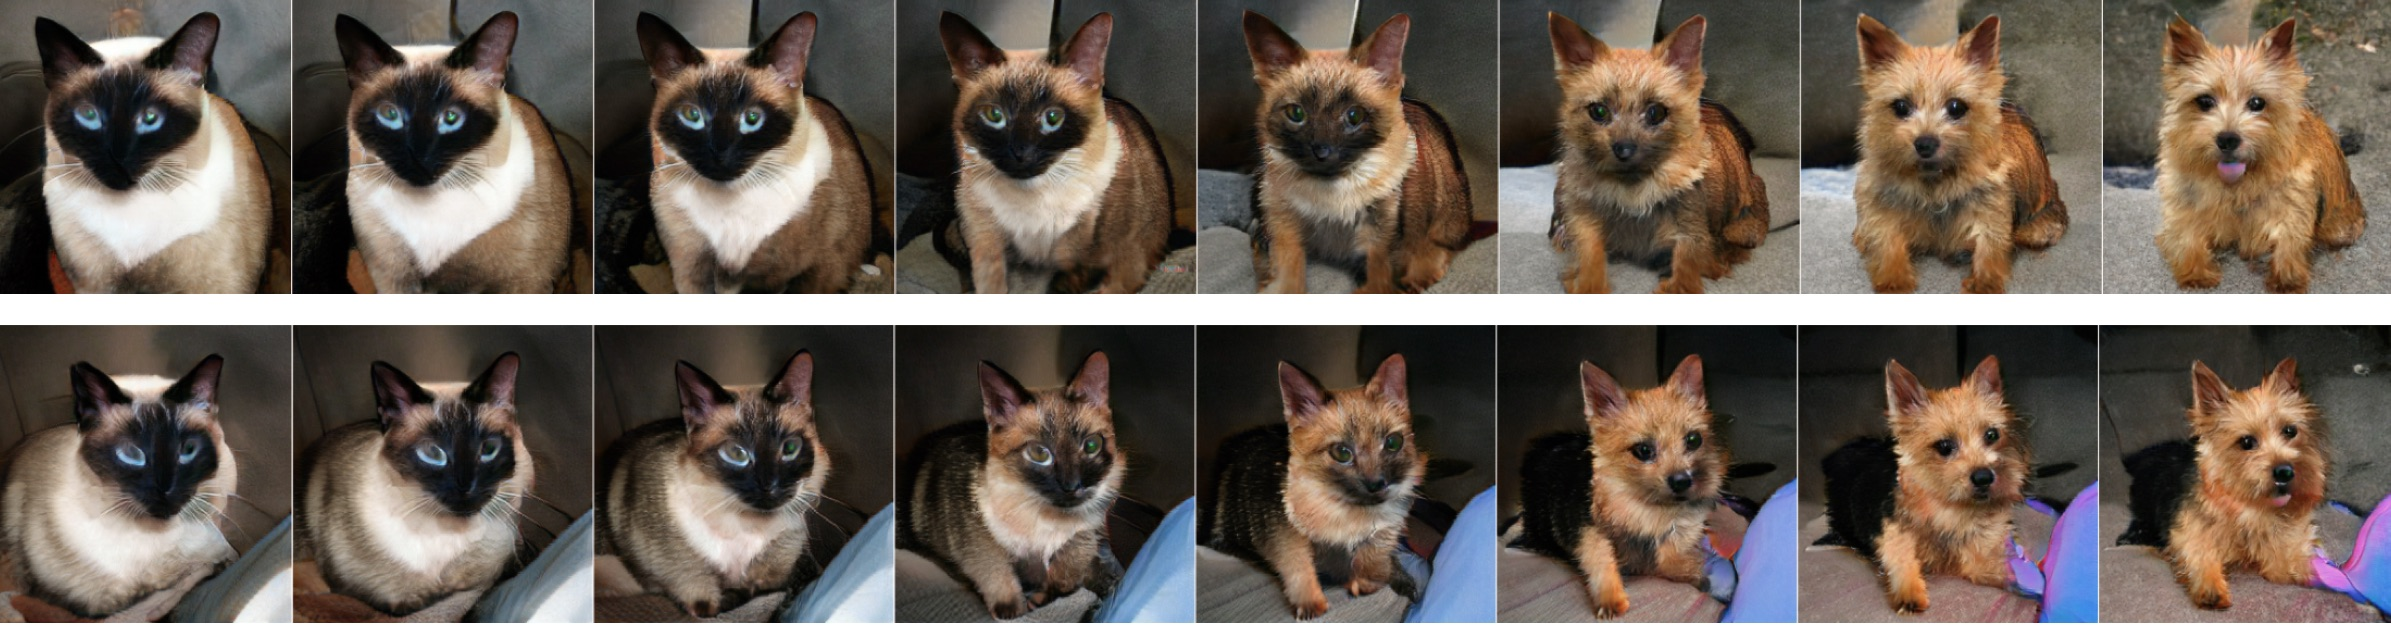
\includegraphics[width=.95\linewidth]{deepfake}
\caption{\label{fig:deepfake} Deux exemples de \guill{deep fakes} qui sont des images virtuelles interpolant entre chats et chiens. }
\end{figure}


